\section{Limitations of the flatness-based analysis in \ood}%
\label{app:limit_proof_swad}%
\begin{theorem}[Equation 21 from \cite{cha2021wad}, simplified version of their Theorem 1]
    Consider a set of $N$ covers $\left\{\Theta_{k}\right\}_{k=1}^{N}$ \sut the parameter space $\Theta \subset \cup_{k}^{N} \Theta_{k}$ where $\operatorname{diam}(\Theta)\triangleq\sup _{\theta, \theta^{\prime} \in \Theta}\left\|\theta-\theta^{\prime}\right\|_{2}, N\triangleq\left\lceil(\operatorname{diam}(\Theta) / \gamma)^{d} \right\rceil$ and $d$ is the dimension of $\Theta$. Then, $\forall\theta \in \Theta$ with probability at least $1-\delta$:
    \begin{equation} \label{eq:bound_swad}
        \begin{aligned}
            \mathcal{E}_{T}(\theta) & \leq \frac{1}{2} \operatorname{Div}(p_S, p_T) + \mathcal{E}_{S}(\theta)                                                                                                                    \\
                                   & \leq \frac{1}{2} \operatorname{Div}(p_S, p_T) + \mathcal{E}_{d_S}^{\gamma}(\theta)+\max _{k} \sqrt{\frac{\left(v_{k}\left[\ln \left(n_S / v_{k}\right)+1\right]+\ln (N / \delta)\right)}{2 n_S}},%
        \end{aligned}%
    \end{equation}%
    where:
    \begin{itemize}%
        \vspace{-0.5em}%
        \item $\mathcal{E}_{T}(\theta) \triangleq \mathbb{E}_{(x,y)\sim p_T(X,Y)}[\ell\left(f_\theta(x);y\right)]$ is the expected risk on the target domain,
        \item $\operatorname{Div}(p_S, p_T) \triangleq 2 \sup _{A}\left|p_{S}(A)-p_{T}(A)\right|$ is a divergence between the source and target marginal distributions $p_S$ and $p_T$: it measures diversity shift.%
        \item $\mathcal{E}_{S}(\theta) \triangleq \mathbb{E}_{(x,y)\sim p_S(X,Y)}[\ell\left(f_\theta(x);y\right)]$ is the expected risk on the source domain,
        \item $\mathcal{E}_{d_S}^{\gamma}(\theta) \triangleq \max _{\|\Delta\| \leq \gamma} \mathcal{E}_{d_S}(\theta+\Delta)$
        (where $\mathcal{E}_{d_S}(\theta+\Delta) \triangleq \mathbb{E}_{(x,y)\in d_S}[\ell\left(f_{\theta+\Delta}(x);y\right)]$)
        is the robust empirical loss on source training dataset $d_S$ from $S$ of size $n_S$,
        \item $v_{k}$ is a VC dimension of each $\Theta_{k}$.%
    \end{itemize}%
    \label{theorem:swad}%
    \vspace{-0.5em}%
\end{theorem}%
Previous understanding of WA's success in \ood relied on this upper-bound, where $\mathcal{E}_{d_S}^{\gamma}(\theta)$ involves the solution's flatness.
This is usually empirically analyzed by the trace of the Hessian \cite{pmlr-v70-dinh17b,petzka2021relative,yao2020pyhessian}: indeed, with a second-order Taylor approximation around the local minima $\theta$ and $h$ the Hessian's maximum eigenvalue, $\mathcal{E}_{d_S}^{\gamma}(\theta) \approx \mathcal{E}_{d_S}(\theta) + h \times \gamma^2$.

In the following subsections, we show that this inequality does not fully explain the exceptional performance of WA on DomainBed \cite{gulrajani2021in}. Moreover, we illustrate that our bias-variance-covariance-locality addresses these limitations.
\subsection{Flatness does not act on distribution shifts}
\label{app:flatness_distribution_shifts}
% does not predict under which circumstances WA would work
The flatness-based analysis is not specific to \ood.
Indeed, the upper-bound in \Cref{eq:bound_swad} sums up two noninteracting terms: a domain divergence $\mathrm{Div}(p_S,p_T)$ that grows in \ood and $\mathcal{E}_{d_S}^{\gamma}(\theta)$ that measures the \iid flatness.
The flatness term can indeed be reduced empirically with WA: yet, it does not tackle the domain gap.
In fact, \Cref{eq:bound_swad} states that additional flatness reduces the upper bound of the error similarly no matter the strength of the distribution shift, thus as well \ood than \iid.
In contrast, our analysis shows that variance (which grows with diversity shift, see \Cref{subsec:expression_ood_var}) is tackled for large $M$: our error is controlled even under large diversity shift. This is consistent with our experiments in \Cref{table:db_all_training}.
Our analysis also explains why WA cannot tackle correlation shift (where bias dominates, see \Cref{app:failure_corr_shift}), a limitation \cite{cha2021wad} does not illustrate.

\subsection{SAM leads to flatter minimas but worse \ood performance}
\label{app:mav_better_than_sam}
The flatness-based analysis does not explain why WA outperforms other flatness-based methods in \ood.
We consider Sharpness-Aware Minimizer (SAM) \cite{foret2021}, another popular method to find flat minima based on minimax optimization: it minimizes the maximum loss around a neighborhood of the current weights $\theta$.
In \Cref{fig:soup:boxplot_masam}, we compare the flatness (\ie the Hessian trace computed with the package in \cite{yao2020pyhessian}) and accuracy of ERM, MA \cite{arpit2021ensemble} (a WA strategy) and SAM \cite{foret2021} when trained on the \enquote{Clipart}, \enquote{Product} and \enquote{Photo} domains from OfficeHome \cite{venkateswara2017deep}: they are tested \ood on the fourth domain \enquote{Art}.
Analyzing the second and the third rows of \Cref{fig:home0:boxplot_masam_train_hess,fig:home0:boxplot_masam_ood_hess}, we observe that SAM indeed finds flat minimas (at least comparable to MA), both in training (\iid) and test (\ood). However, this is not reflected in the  \ood accuracies in \Cref{fig:soup:boxplot_masam_ood_acc}, where MA outperforms SAM.
As reported in \Cref{table:db_swad_all}, similar experiments across more datasets lead to the same conclusions in \cite{cha2021wad}.
In conclusion, flatness is not sufficient to explain why WA works so well in \ood, because SAM has similar flatness but worse \ood results.
In contrast, we highlight in this paper that WA succeeds in \ood by reducing the impact of variance thanks to its similarity with prediction ensembling \cite{Lakshminarayanan2017} (see \Cref{lemma:wa_ensembling}), a privileged link that SAM does not benefit from.%
% \clearpage
\begin{table}[h]%
    \caption{\textbf{Accuracy ($\uparrow$) on DomainBed for SWAD}, taken from Table 4 in \cite{cha2021wad}}%
    \centering
    \adjustbox{width=0.9\textwidth}{
        \begin{tabular}{lccccc|c}
            \toprule
                       & \textbf{PACS}  & \textbf{VLCS}  & \textbf{OfficeHome} & \textbf{TerraInc} & \textbf{DomainNet} & \textbf{Avg}. ( $\Delta)$ \\
            \midrule
            ERM        & 85.5 $\pm$ 0.2 & 77.5 $\pm$ 0.4 & 66.5 $\pm$ 0.3      & 46.1 $\pm$ 1.8    & 40.9 $\pm$ 0.1     & 63.3                      \\
            SWAD \cite{cha2021wad} + ERM & \textbf{88.1} $\pm$ 0.1 & 79.1 $\pm$ 0.1 & \textbf{70.6} $\pm$ 0.2      & \textbf{50.0} $\pm$ 0.3    & \textbf{46.5} $\pm$ 0.1     & \textbf{66.9}(+3.6)                \\
            \midrule
            SAM \cite{foret2021}        & 85.8 $\pm$ 0.2 & \textbf{79.4} $\pm$ 0.1 & 69.6 $\pm$ 0.1      & 43.3 $\pm$ 0.7    & 44.3 $\pm$ 0.0     & 64.5                      \\
            SWAD \cite{cha2021wad} + SAM \cite{foret2021} & 87.1 $\pm$ 0.2 & 78.5 $\pm$ 0.2 & 69.9 $\pm$ 0.1      & 45.3 $\pm$ 0.9    & \textbf{46.5} $\pm$ 0.1     & 65.5(+1.0)                \\
            \bottomrule
        \end{tabular}
    }
    \label{table:db_swad_all}%
\end{table}%
%
\FloatBarrier
\clearpage
\begin{figure}[t]%
    \centering%
    \begin{subfigure}{.33\textwidth}%
        \centering%
        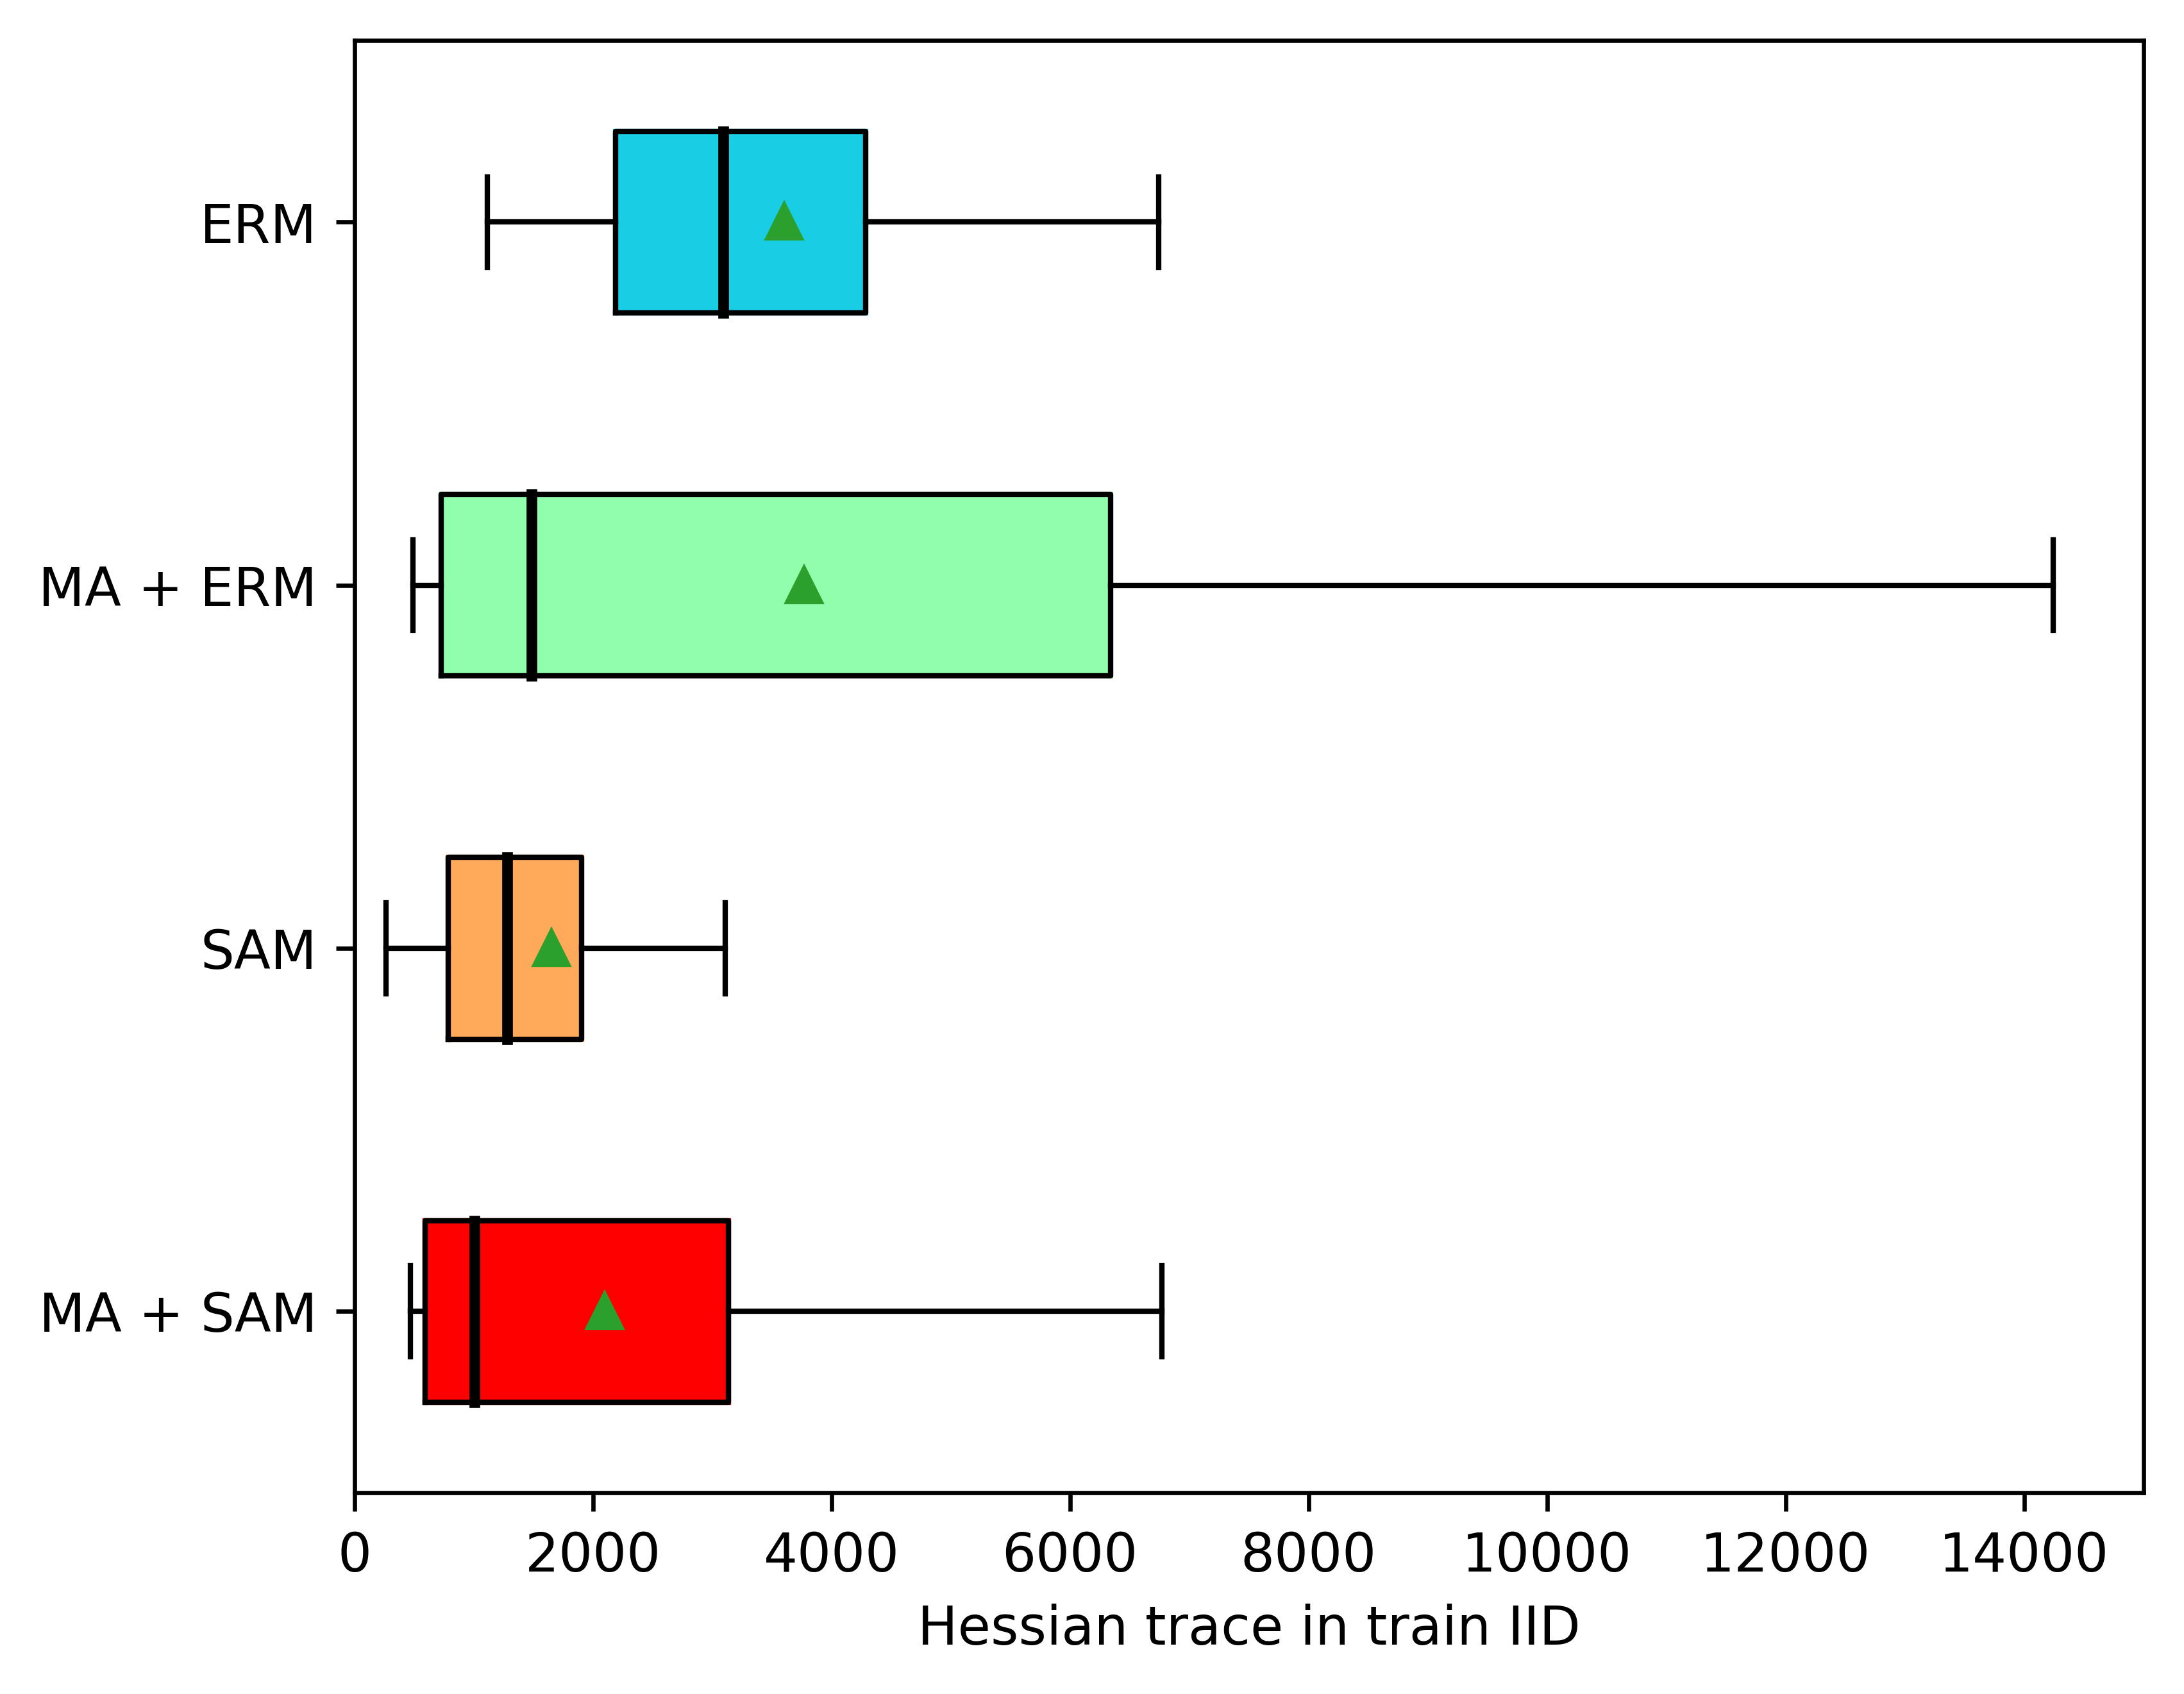
\includegraphics[width=\linewidth]{pictures/files/final/boxplot_masam_train_hess.png}%
        \caption{Hessian trace ($\downarrow$) in train.}%
        \label{fig:home0:boxplot_masam_train_hess}%
    \end{subfigure}%
    \begin{subfigure}{.33\textwidth}%
        \centering%
        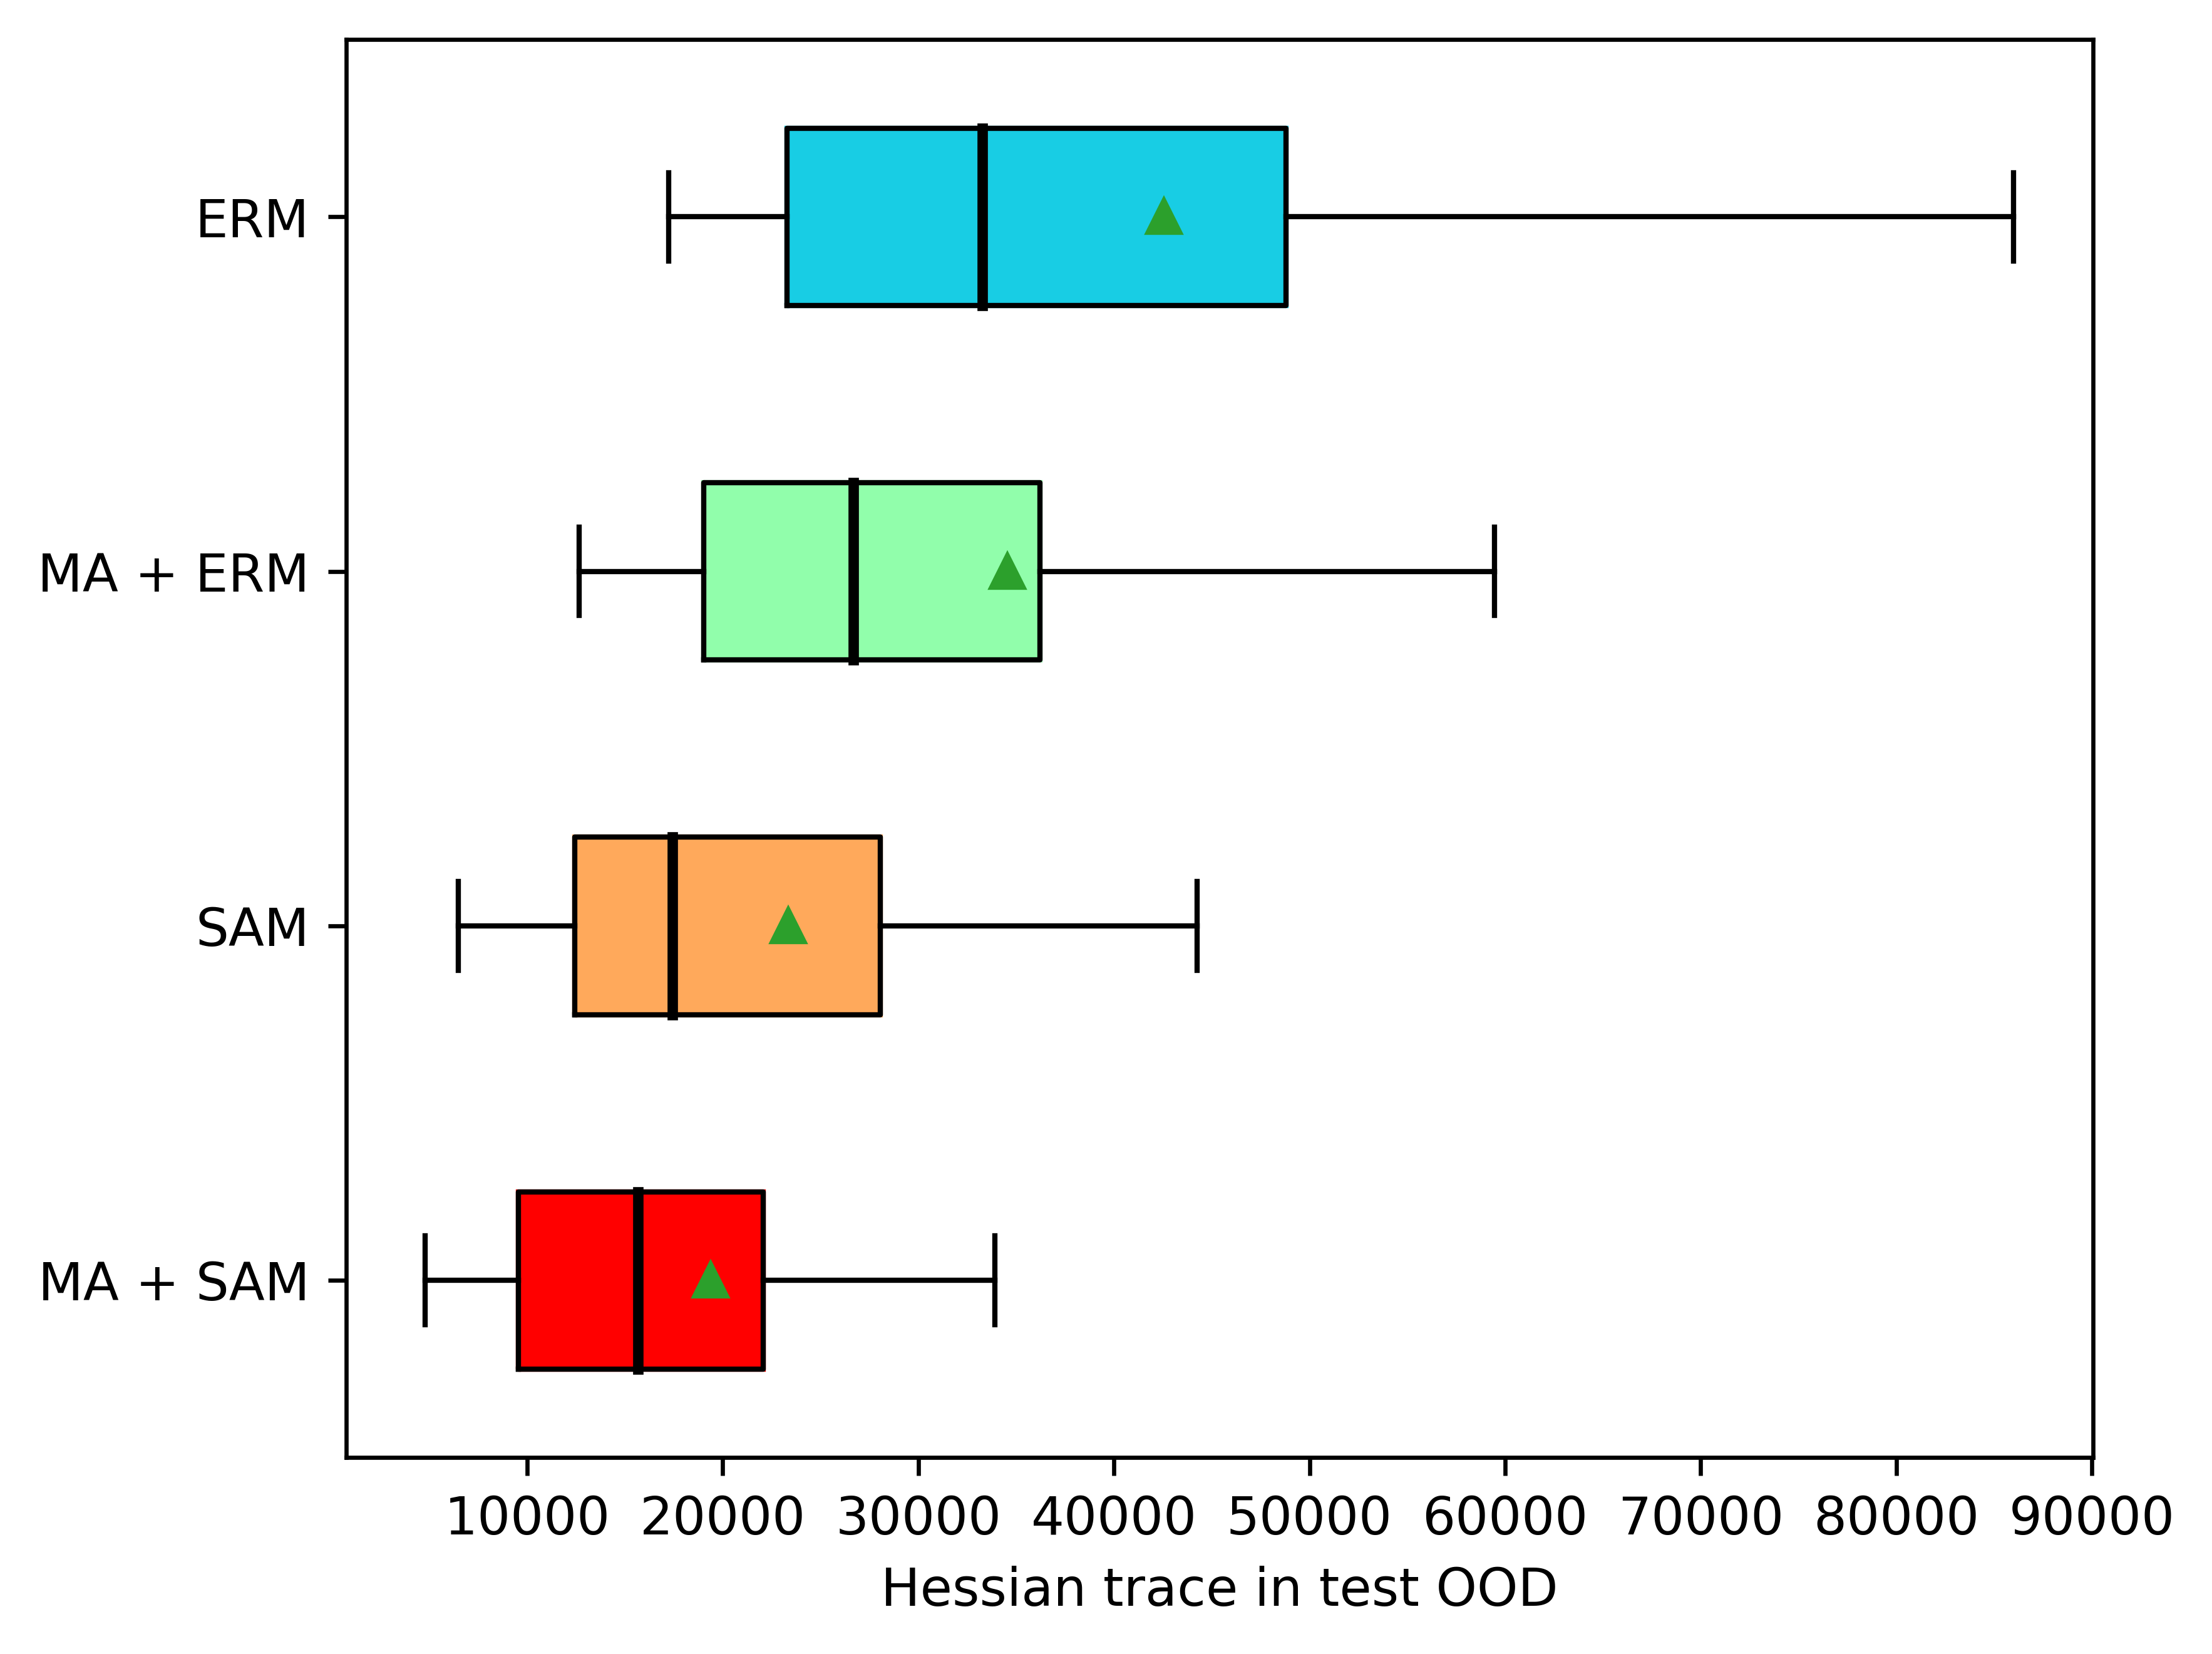
\includegraphics[width=\linewidth]{pictures/files/final/boxplot_masam_ood_hess.png}%
        \caption{Hessian trace ($\downarrow$) in test \ood.}%
        \label{fig:home0:boxplot_masam_ood_hess}%
    \end{subfigure}%
    \begin{subfigure}{.33\textwidth}%
        \centering%
        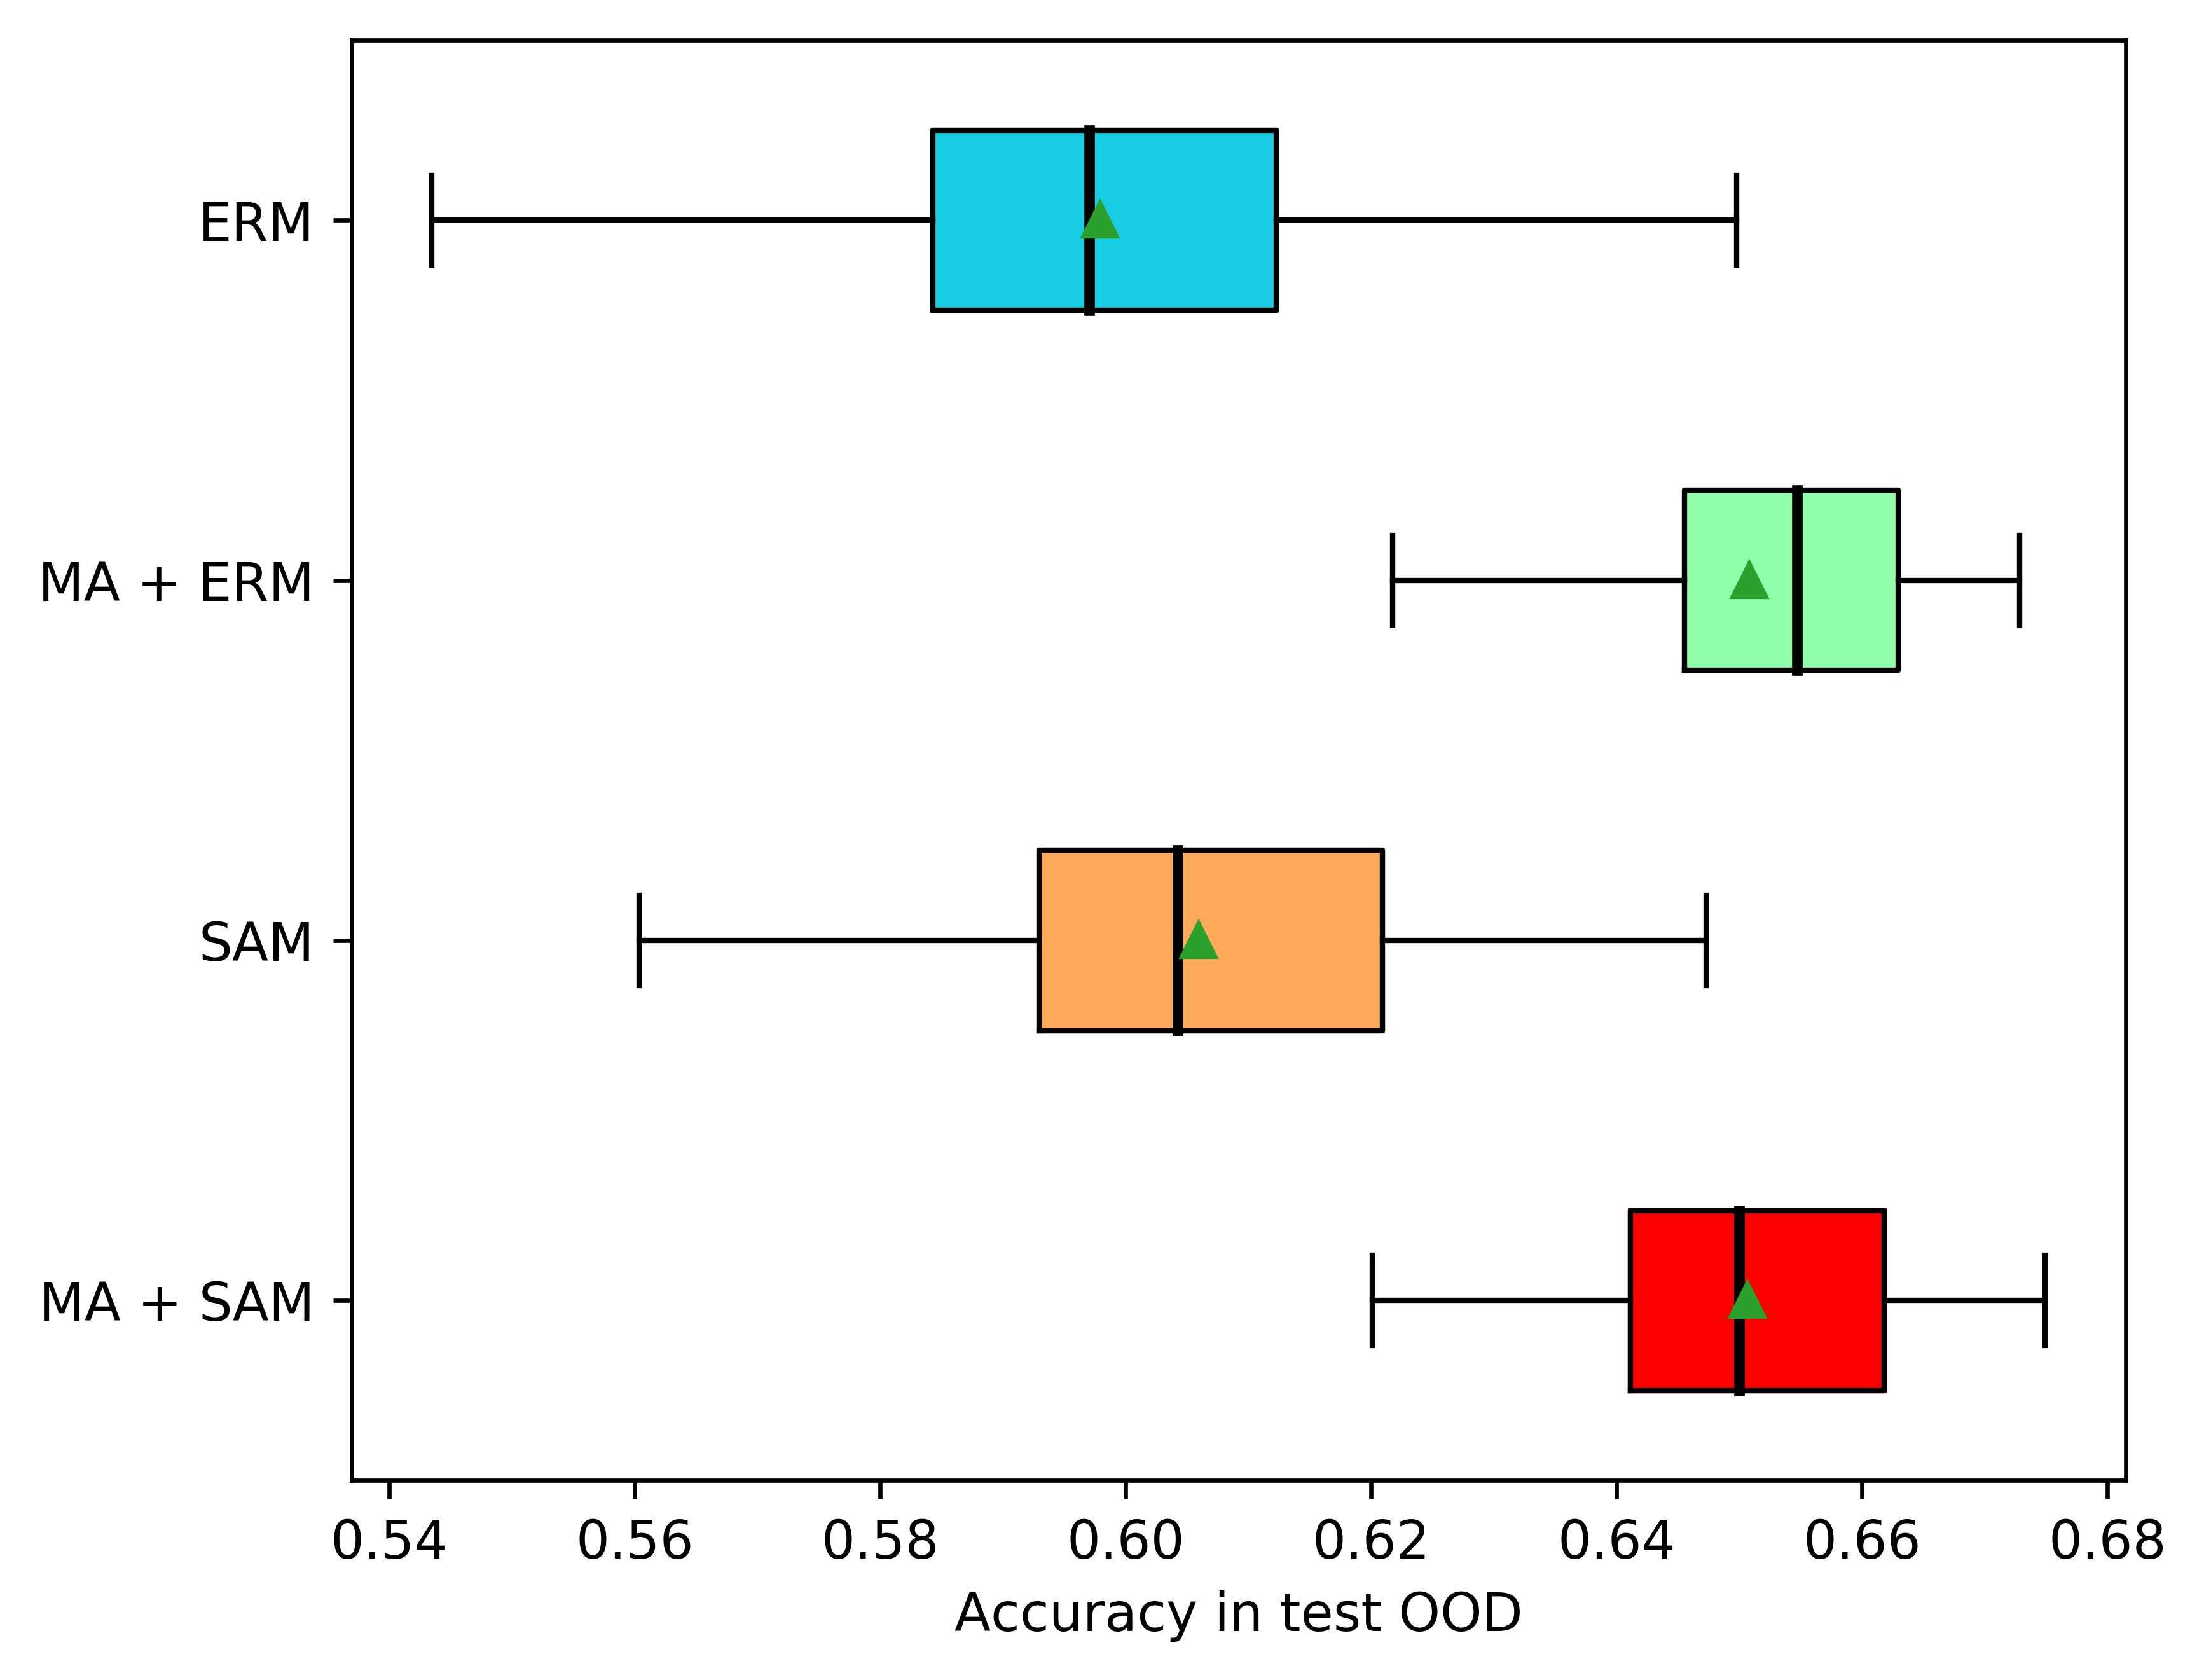
\includegraphics[width=\linewidth]{pictures/files/final/boxplot_masam_ood_acc.png}%
        \caption{Accuracy ($\uparrow$) in test \ood.}
        \label{fig:soup:boxplot_masam_ood_acc}%
    \end{subfigure}%
    \caption{MA \cite{arpit2021ensemble} (a WA strategy) and SAM \cite{foret2021} similarly improve flatness. When combined, they further improve flatness. Yet, MA outperforms SAM and beats MA + SAM in \ood accuracy on domain \enquote{Art} from OfficeHome.}%
    \label{fig:soup:boxplot_masam}%
\end{figure}%
%
\begin{table}[h]%
    \caption{\reb{\textbf{Accuracy ($\uparrow$) impact of including SAM} on domain \enquote{Art} from OfficeHome.}}
    \centering
    \adjustbox{width=0.7\textwidth}{
        \reb{\begin{tabular}{llll}
            \toprule
            \textbf{Algorithm}          & \textbf{Weight selection} & ERM            & SAM \cite{foret2021} \\
            \midrule
            No DiWA                         & N/A                       & 62.9 $\pm$ 1.3 & 63.5 $\pm$ 0.5       \\
            % MA \cite{arpit2021ensemble} & Uniform                   & 65.0 $\pm$ 0.2 & 65.5 $\pm$ 0.4       \\
            DiWA                        & Restricted: $M \leq 20$   & 66.7 $\pm$ 0.1 & 65.4 $\pm$ 0.1       \\
            DiWA                        & Uniform: $M = 20$         & 67.3 $\pm$ 0.3 & 66.7 $\pm$ 0.2       \\
            DiWA$^{\dagger}$            & Uniform: $M = 60$         & \textbf{67.7}           & \textbf{67.4}                 \\
            \bottomrule
        \end{tabular}}}
    \label{table:db_home0_sam}%
\end{table}

\subsection{WA and SAM are not complementary in \ood when variance dominates}%
\begin{wrapfigure}[20]{hR!}{0.34\textwidth}
    \vspace{-0.5em}%
    \centering%
    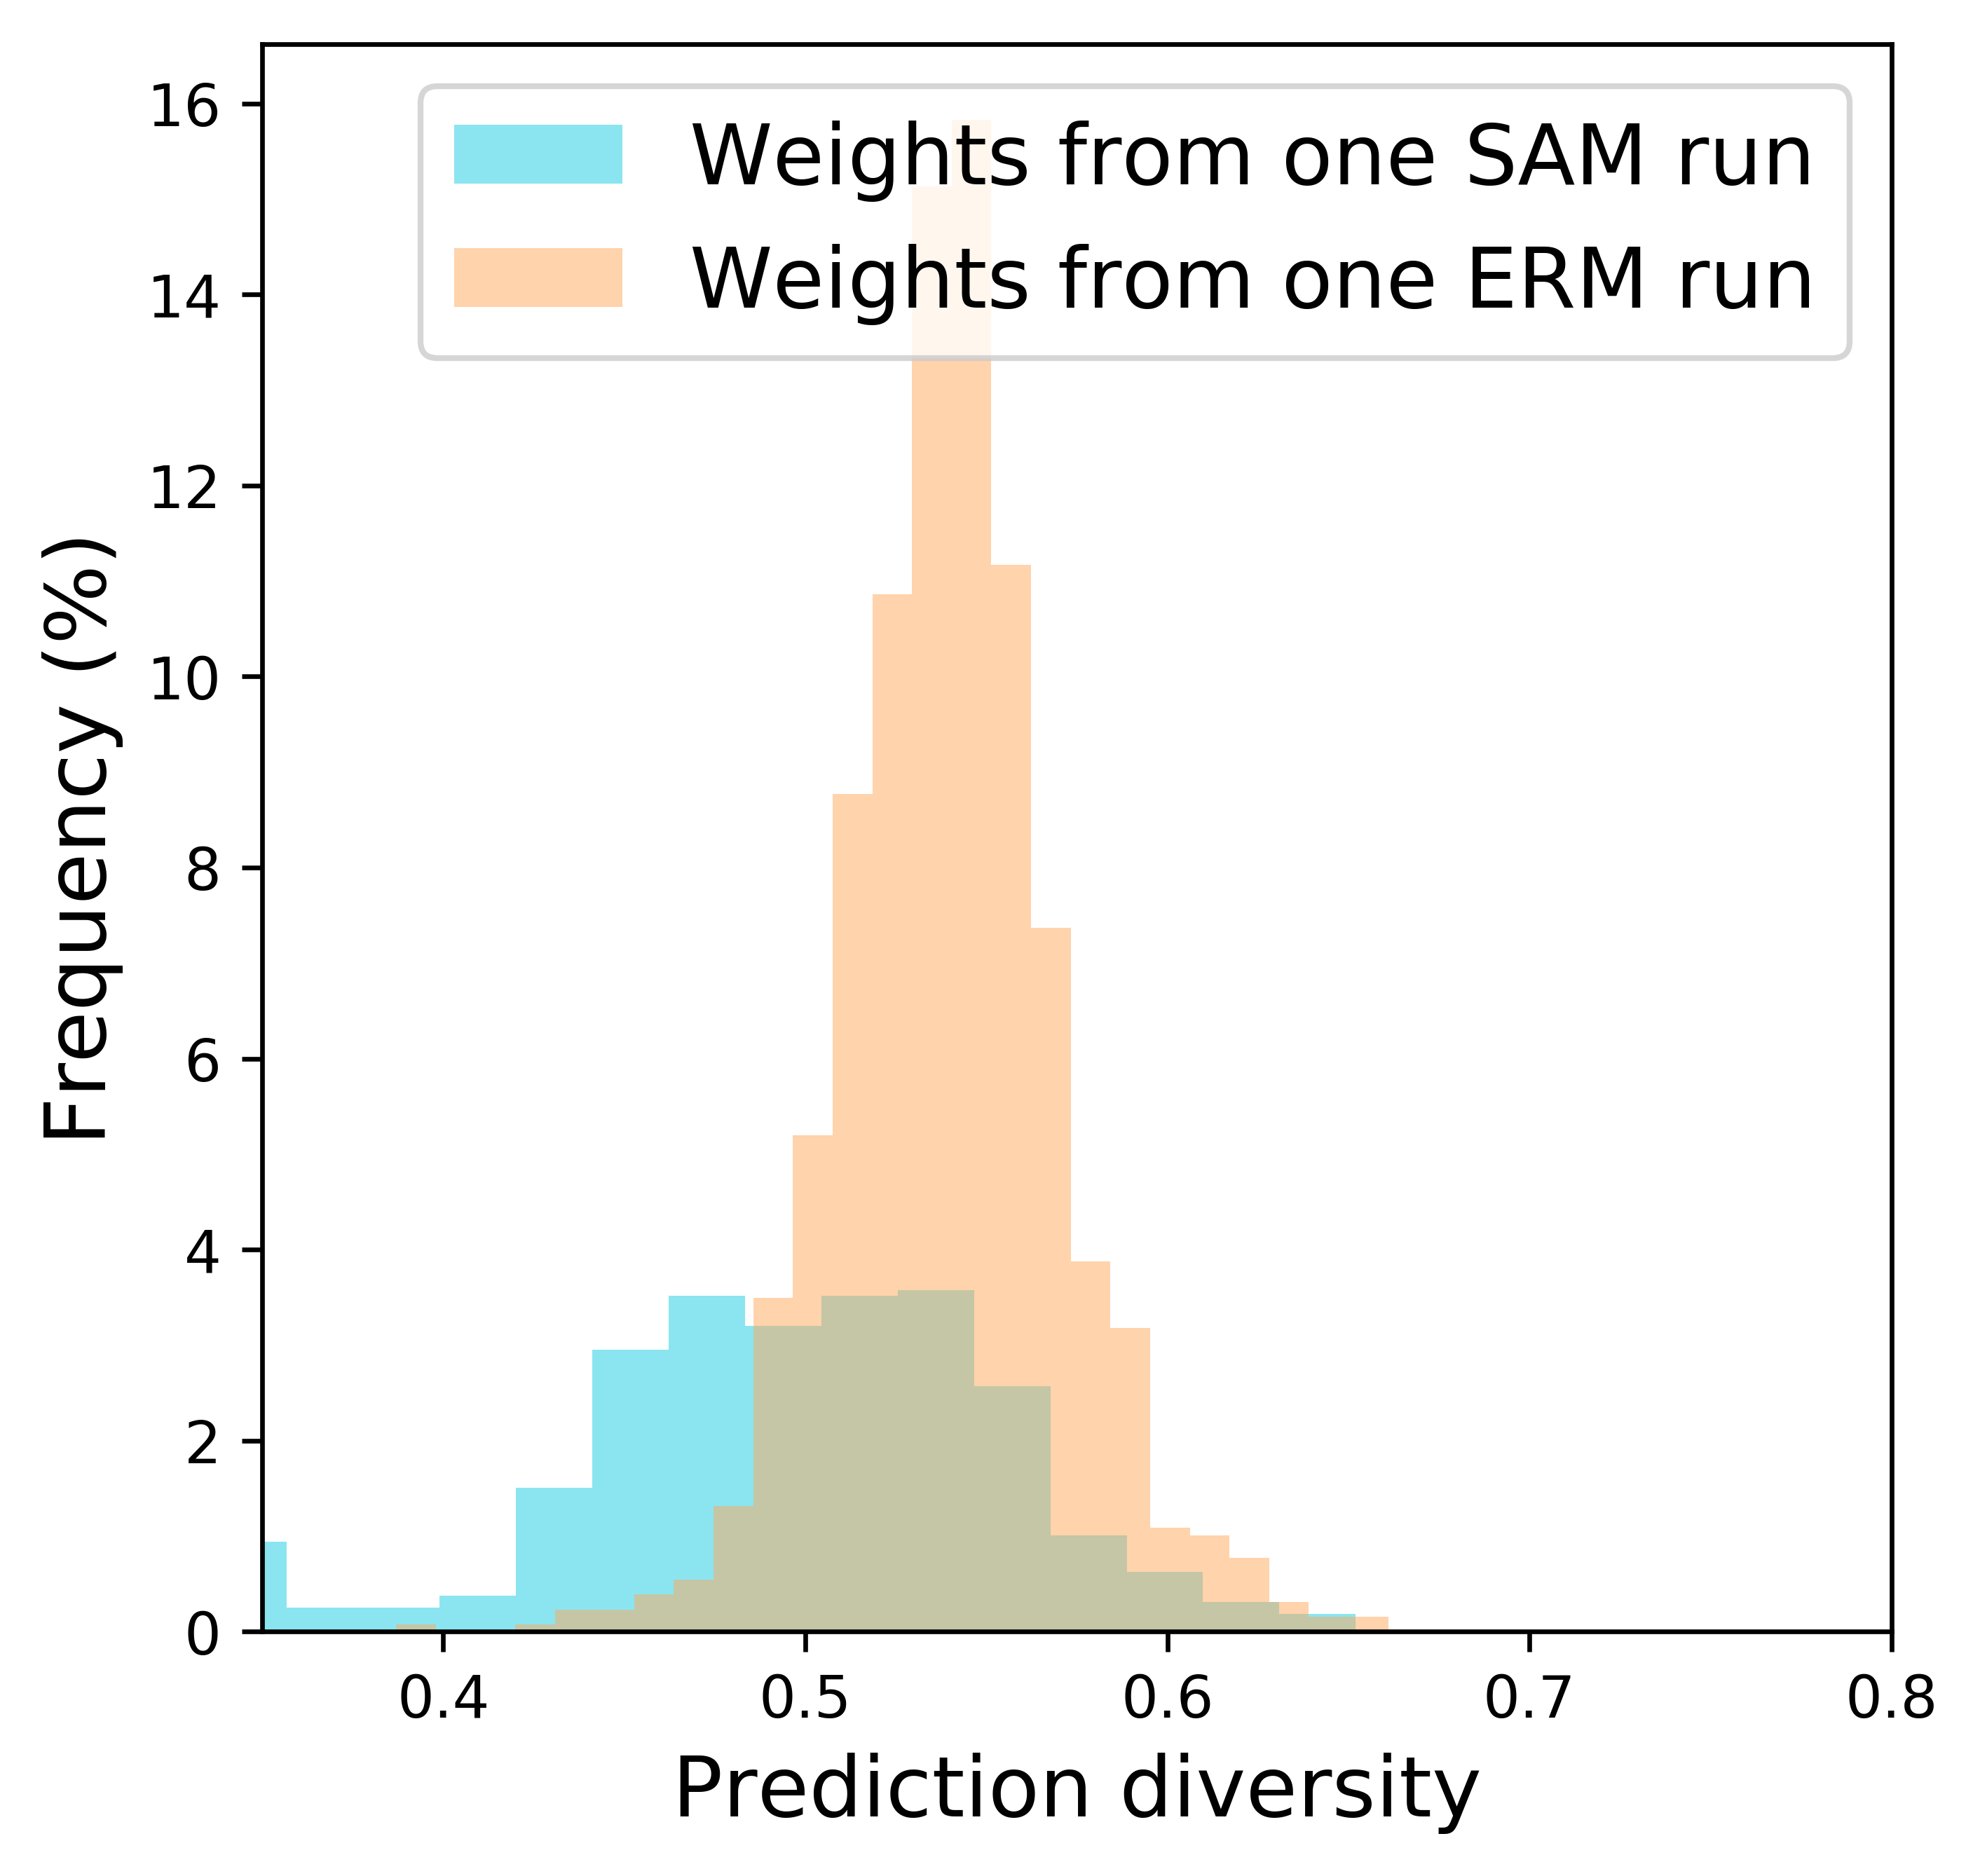
\includegraphics[width=0.34\textwidth]{pictures/files/final/home0_hist_ermsam_dr.png}%
    \caption{Prediction diversity in ratio-error \cite{aksela2003comparison} ($\uparrow$) on domain \enquote{Art} from OfficeHome. Checkpoints along a SAM run are less diverse than along an ERM run.}%
    \label{fig:home0_hist_ermsam_dr}%
    % \vspace{-3em}
\end{wrapfigure}%
%
\label{app:mav_sam_failure}
We investigate a similar inconsistency when combining these two flatness-based methods.
As argued in \cite{questionsflatminima22}, we confirm in \Cref{fig:home0:boxplot_masam_train_hess,fig:home0:boxplot_masam_ood_hess} that MA + SAM leads to flatter minimas than MA alone (\ie with ERM) or SAM alone.
Yet, MA does not benefit from SAM in \Cref{fig:soup:boxplot_masam_ood_acc}.
\cite{cha2021wad} showed an even stronger result in \Cref{table:db_swad_all}: SWAD + ERM performs better than SWAD + SAM.
\reb{We recover similar findings in \Cref{table:db_home0_sam}: DiWA performs worse when SAM is applied in each training run}.

This behavior is not explained by \Cref{theorem:swad}, which states that more flatness should improve \ood generalization. Yet it is explained by our diversity-based analysis.
Indeed, we observe in \Cref{fig:home0_hist_ermsam_dr} that the diversity across two checkpoints along a SAM trajectory is much lower than along a standard ERM trajectory (with SGD).
We speculate that this is related to the recent empirical observation made in \cite{dallev2}: \enquote{the rank of the CLIP representation space is drastically reduced when training CLIP with SAM}.
Under diversity shift, variance dominates (see \Cref{eq:int_var}): in this setup, the gain in accuracy of models trained with SAM cannot compensate the decrease in diversity. This explains why WA and SAM are not complementary under diversity shift: in this case, variance is large.
% In contrast, they were shown to be complementary in \iid \cite{questionsflatminima22} where the variance is smaller \cite{neal2018modern,belkin2019reconciling,pmlr-v119-d-ascoli20a}.
% Under diversity shift, variance dominates (see \Cref{eq:int_var}) such that covariance may be high (due to Cauchy Schwartz inequality covariance is smaller to variance \cf proof in \Cref{app:proof_wa_ind}).
% Then covariance is also small such that the loss of diversity due to SAM does not have a big impact of performance.
\FloatBarrier
\clearpage
